%
%

\pdfbookmark[1]{Вступ}{intro}
\section*{Вступ}
Шановні автори, даний документ є прикладом оформлення статті в редакторі \LaTeX\ для публікації у журналі <<Вісник Національного технічного університету України ``Київський політехнічний інститут''. Серія Радіотехніка. Радіоапаратобудування>>. У разі використання запропонованого редакцією шаблону всі правила оформлення будуть застосовані автоматично.

\section{Порядок проходження рукописів статей}
Усі рукописи статей слід подавати через форму на сайті. Для цього необхідно зареєструватися на сайті та пройти 5 кроків слідуючи детальним інструкціям. У разі якщо у статті оформлені метадані трьома мовами (назва, анотація, ключові слова, прізвища авторів у транслітерації) процес подання займе не більше 5-ти хвилин. Формат документів, у якому подається рукопис на рецензування може бути: \texttt{*.pdf}, \texttt{*.tex}, \texttt{*.doc}. Розмір не повинен перевищувати 4 МБ. Проте у разі успішного проходження рецензування рукопис слід оформити у редакторі \LaTeX\ з використанням запропонованого редакцією стильового файлу.

Проходження статей до друку відбувається у декілька етапів:
\begin{list}{-}{}
	\item реєстрація подання через сайт \texttt{radap.kpi.ua};
	\item рецензування (до 2-х місяців);
	\item літературна корекція;
	\item редакторська підготовка;
	\item публікація випуску.
\end{list}  

Періодичніть друку 4-ри рази на рік: 
\begin{enumerate}
	\begin{multicols}{2}
	\item 30 березня, 
	\item 30 червня, 
	\item 30 вересня, 
	\item 30 грудня.
	\end{multicols}
\end{enumerate}

\section{Вимоги до оформлення}

Статті повинні мати такі необхідні елементи: 
\begin{list}{-}{}
	\item постановка задачі; 
	\item аналіз досліджень і публікацій, в яких започатковано розв'язання даної задачі; 
	\item виділення невирішених частин загальної проблеми, котрим присвячується означена стаття; 
	\item формулювання цілей статті; 
	\item виклад матеріалу дослідження; 
	\item обговорення (аналіз) приведених у статті результатів, порівняння з результатами інших дослідників; 
	\item висновки з даного дослідження, перспективи його подальшого розвитку.
\end{list}

У зв'язку з цим науково-технічні статті та повідомлення про досягнення науково-практичних результатів мають бути структурованими - поділеними на розділи з заголовками. Наприклад, для науково-технічних статей: вступ, постановка задачі, теоретичні викладки, методика та засоби експериментальних досліджень, принципи побудови та схемно-конструкторські особливості розробленої апаратури, результати експериментів та випробувань розробленої апаратури, обговорення та оцінка отриманих результатів з вже відомими, висновки та рекомендації.

Статті можуть бути опубліковані однією  з трьох мов --- українською, російською, англійською. Проте метадані (Назва, анотація, ключові слова) надаються трьома мовами (українською, російською та англійською). Обсяг анотації 10 - 12 рядків. Англійська анотація має бути розширеною та структурованою відповідно до структури статті з відображенням основних отриманих результатів.

Обсяг рукопису має становити 5 -- 7 повних сторінок формату А4 (включаючи рисунки, таблиці, перелік посилань, анотації та ключові слова).

У рукописах слід дотримуватись термінології, прийнятої державними стандартами; у разі використання нових термінів або абревіатур, слід їх розшифрувати та пояснити у тексті.



\section{Приклади оформлення окремих елементів статті}


\subsection{Формули}
Формули можуть розміщуватися у тексті: $\mathbf{\eta}_0$, $E\left\lbrace \hat{\mathbf{\eta}}\right\rbrace = \mathbf{\eta}_0$ або їх можна виокремити окремим рядком.  Для того, щоб можливо було оформити посилання на формулу, слід використовувати мітки, наприклад: \texttt{$\backslash$label\{eq1\}}. Далі зробити посилання на це рівняння можна за допомогою виразу: \texttt{$\backslash$eqref\{eq1\}}. Таким чином можливо здійснити автоматичну нумерацію формул.

\begin{equation}\label{eq1}
H(A)=-\sum \limits_{i=1}^n p_i \log p(p_i)
\end{equation}


Декілька рівнянь з позначкою одним номером:
\begin{equation}
\begin{aligned}\label{eq2}
\rho_{+mn}^E &=\frac{Z_0-Z_{B_{mn}}^E}{Z_0-Z_{mn}^E} =-\rho_{+mn}^H \\
\rho_{+mn}^H &=\frac{\sqrt{1-\left( \frac{m\lambda}{2b_p}\right) ^2-\left( \frac{m\lambda}{2a_p}\right) ^2}-1 }{\sqrt{1-\left( \frac{m\lambda}{2b_p}\right) ^2-\left( \frac{m\lambda}{2a_p}\right) ^2}+1}
\end{aligned}
\end{equation}

Довгі формули слід записувати у декілька стрічок як це приведено нижче:
\begin{multline}\label{radap1345eq2}
U_{i-1}= \sum\limits_{j=0}^{i-1}\left| r_j - \sum\limits_{h=0}^{g} x_{(j-h)} \nu_h \right|^2 =\\= \sum\limits_{j=0}^{i-2}\left| r_j - \sum\limits_{h=0}^{g} x_{(j-h)} \nu_h \right|^2 +w_{i-1} =\\= U_{i-2} + w_{i-1} 
\end{multline}

Дуже довгі формули, що варко розмістити в одній колонці можна розмістити на всю сторінку як це приведено нижче:

\end{multicols} % Закриваємо розмітку на дві колонки

\begin{align}\label{radap1333eq17} % Формула на всю сторінку
\begin{split}
A_{+m_x m_y}^{H_\perp} \cong -4E_0a_pe^{-inkd_y\sin\theta_П}\frac{a_p(1+\cos \theta_П)}{(m_y\pi)^2} 
\frac{\sin^2{(\frac{m_y\pi}{2})}\cos{(\frac{ka_p}{2}\sin{\theta_П})}+i\cos^2{(\frac{m_y\pi}{2})}\sin{(\frac{ka_p}{2}\sin{\theta_П})}}{\left( 1+\sqrt{1-\left( \frac{m_y\lambda}{2a_p}\right) ^2}\right) \left( 1-\rho_{-mn}^H \rho_{+mn}^H \left( 1-\left( \frac{2a_p}{m_y\lambda}\sin\theta_П\right) ^2\right) \right)  }
\end{split}	 
\end{align}	

\begin{multicols}{2} % Відкриваємо нову розмітку на дві колонки


\subsection{Рисунки}
Всі рисунки в статті бажано оформляти у векторному вигляді і зберігати їх в форматі \texttt{.pdf}. Оформити векторні рисунки можливо у програмах \textit{Visio}, \textit{Corel~Draw}, \textit{Microsoft Office}, \textit{TikZ} та ін. Також можливо вставляти растрові малюнки у форматі \texttt{*.png} або \texttt{*.jpeg} з якістю, що є достатньою для якісного друку (не менше \texttt{300dpi}). Файли рисунків мають бути розміщені в одній директорії з текстовим файлом. Маштабування задається як параметр до команди вставки рисунку. Приклади вставки рисунків приведено на рис. \ref{fig1} та \ref{fig2}. Мітки для рисунків оформляються агналогічно формулам, автоматичні посилання на рbсунок можливо здійснити командою \texttt{$\backslash$ref\{label\}}.


\begin{Figure}\centering%{l}{\linewidth}
	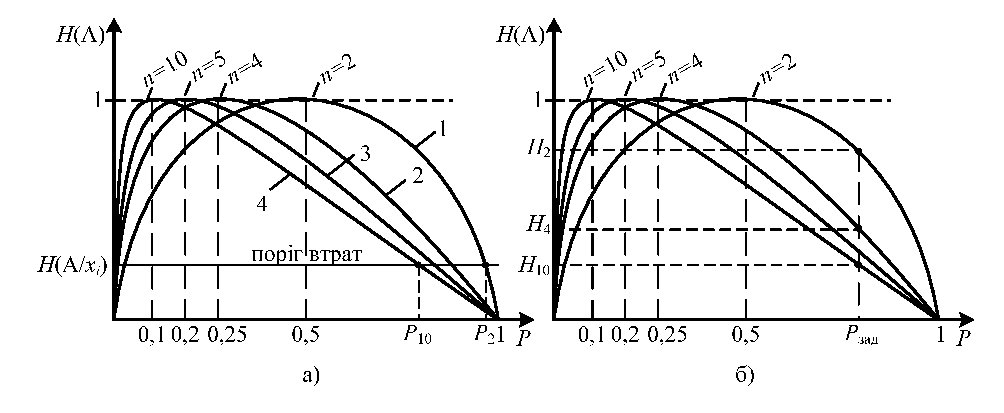
\includegraphics[width=\linewidth]{fig1}
	\captionof{figure}{Підпис до рисунку}\label{fig1}
\end{Figure}

\begin{figure*}\centering
	%Figure 5 	
	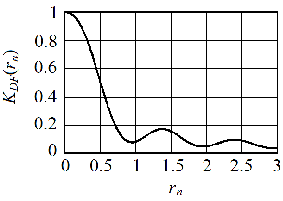
\includegraphics[width=0.4\linewidth]{fig2a}
	~~~~~
	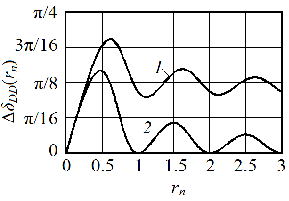
\includegraphics[width=0.4\linewidth]{fig2b}
	\begin{tabular}{p{0.49\linewidth}p{0.49\linewidth}}
		\centering (a) & \centering (b)  
	\end{tabular}	
	\captionof{figure}{Підпис до рисунку (a) $\Delta\delta_{DD}(r_n)$ (b)  $\theta = 1 $}\label{fig2}%
\end{figure*}



\subsection{Таблиці}

Таблиці можуть мати заголовок, розміщений над таблицею. 
\begin{Table}
	\captionof{table}{Заголовок таблиці}
	\begin{tabularx}{\linewidth}{|l|X|c|}
		\hline 
		\rule{0pt}{11pt} $\mathrm{const}$ & $\tilde{K}$ &  $S$\\ 
		\hline 
		\rule{0pt}{10pt}$p=0,001$& $1,2359\times V^{0,1241}-1,3399$ &  0,00158\\ 
		\hline 
		\rule{0pt}{10pt}$p=0,005$& $-8,3753\times V^{-0,0274}+8,2477$ &  0,00150\\ 
		\hline 
		\rule{0pt}{10pt}$p=0,01$&  $2,7669\times V^{-0,0983}+2,6440$&  0,00092\\ 
		\hline 
		\rule{0pt}{10pt}$p=0,02$&  $-1,8264\times V^{-0,1769}+1,7115$&  0,00072\\ 
		\hline 
		\rule{0pt}{10pt}$p=0,05$&  $-1,3804\times V^{-0,2872}+1,3013$&  0,00045\\ 
		\hline 
		\rule{0pt}{10pt}$p=0,001$&  $1,6368\times Z^{0,736}-1,4640$&  0,00023\\ 
		\hline 
		\rule{0pt}{10pt}$p=0,005$&  $3,1652\times Z^{0,0420}-2,9549$&  0,00041\\ 
		\hline 
		\rule{0pt}{10pt}$p=0,01$&  $-6,2994\times Z^{-0,0244}+6,5212$&  0,00031\\ 
		\hline 
		\rule{0pt}{10pt}$p=0,03$&  $-2,2772\times Z^{-0,0749}+2,5429$&  0,00012\\ 
		\hline 
	\end{tabularx} \label{radap1361tab1}
\end{Table}

\section{Оформлення посилань}

Перелік посилань подається в порядку згадування у тексті та має бути оформлений згідно ДСТУ-ГОСТ 7.1:2006 та у транслітерації стилем Harvard. У разі якщо всі джерела є англомовними посилання слід оформляти без транслітерації, але з використанням стилю Harvard.

Приклад оформлення посилань \cite{radap1354ref1,radap1354ref4}. 



\pdfbookmark[1]{Висновки}{conc}
\section*{Висновки}
Рукопис оформлений відповідно до цього шаблону слід надсилати у редакцію через офіційний сайт, після чого до Вас на електронну пошту прийде підтвердження отримання рукопису. Далі редактор виконає формальну перевірку рукопису на відповідність вимогам до оформлення статей та направить його на рецензування. Матеріали, що оформлені з відхиленнями від встановлених вимог можуть направляютися авторам на доопрацювання. У разі виникнення запитань звертайтесь до редакції за тел. \texttt{+380 44 204 93 29} або електронною поштою \texttt{radap@rtf.kpi.ua}.



\pdfbookmark[1]{Перелік посилань}{lit}
\section*{Перелік посилань}
\begin{enumerate}\footnotesize
		
	\item Аксенов Г. Н. Основы обработки и анализа сигналов РЕС. Основы структурно-системного метода обработки данных радиоизлучений / Г.Н.~Аксенов,  Ю.А.~Смирнов.~--  К.~: КВИРТУ ПВО, 1989.~-- 200 с.
	\item Шуренок В. А. Використання алгоритмів нечіткого кластерного аналізу для забезпечення функціональної стійкості ієрархічного інформаційного процесу на етапі класифікації об’єктів радіомоніторингу / В.А.~Шуренок // Збірник наукових праць Житомирського військового інституту імені С. П. Корольова.~-- 2013.~-- №7.~-- с. 61-69.
	\item Логачев С.В. Дослідження методів ідентифікації радіотехничніх вимірів при супроводі близько розташованих об’єктів / С.В.~Логачев, Г.В.~Худов, Р.В.~Дзюбчук  / Збірник наукових праць Житомирського військового інституту імені С.П. Корольова.~-- 2013.~-- №8.~-- С. 47--53.  
	\item Анисимов Б.В. Распознавание и цифровая обработка изображений  / Б.В.~Анисимов, В.Д.~Курчанов, В.К.~Злобин.~-- М.~: Высшая школа, 1993.~-- 295~с. 
	\item Гриняев С. В.  Борьба сетей /  С. В. Гриняев // Независимое военное обозрение.~-- 2002.~-- №2.~-- с. 11-13.
	\item Таненбаум Э. В. Компьютерные сети, 4-е изд. / Э. В. Таненбаум.~-- СПб.~: Питер, 2015.~-- 992 с.
	\item Вентцель Е.С. Теория вероятностей  /  Е.С.~Вентцель.~-- М.~: Наука, 1969.~-- 576 с.
\end{enumerate}

\pdfbookmark[1]{References}{translit}
\renewcommand{\refname}{References}

\begin{thebibliography}{9}\footnotesize

\bibitem{radap1354ref1} Aksenov G. N. and Smirnov Yu. A. (1989) \textit{Osnovy obrabotki i analiza signalov RES. Osnovy strukturno-sistemnogo metoda obrabotki dannykh radioizluchenii} [Basics of processing and analyzing signals RES. Fundamentals of structural and systematic data processing method of radio emissions], Kyiv, KVIRTU PVO, 200\,p.
\bibitem{radap1354ref2} Shurenok V. A.  (2013) Application of fuzzy cluster analysis algorithms for providing of hierarchical information process functional stability at the stage of radiomonitoring objects classification. \href{http://nbuv.gov.ua/UJRN/Psvz_2013_7_9}{\textit{Problemy stvorennia, vyprobuvannia, zastosuvannia ta ekspluatatsii skladnykh informatsiinykh system}}, No 7, pp. 61-68. (in Ukrainian) 
\bibitem{radap1354ref3} Logachov S. V., Hudov G. V. and Dzуubchuk R. V. (2013) The  research  of  the  methods  for  identification  of radiotechnical measurements accompanied by closely located space objects. \href{http://nbuv.gov.ua/UJRN/Psvz_2013_8_8}{\textit{Problemy stvorennia, vyprobuvannia, zastosuvannia ta ekspluatatsii skladnykh informatsiinykh system}}, No 8, pp. 47-53. (in Ukrainian)  
\bibitem{radap1354ref4} Anisimov B. V., Kurchanov V. D. and Zlobin V. K. (1993) \textit{Raspoznavanie i tsifrovaya obrabotka zobrazhenii} [The recognition and the digital Imaging],  Moskow, Vysshaya shkola, 295\,p. 
\bibitem{radap1354ref5} Grinyaev S. V. (2002) \textit{Bor'ba setei} [Fight of Networks]. Nezavisimoe voennoe obozrenie, No 2, pp. 11-13.
\bibitem{radap1354ref6} Tanenbaum E. V. (2015) \textit{Komp'yuternye seti} [Computer networks]. SPb., Piter, 992\,p.
\bibitem{radap1354ref7} Venttsel' E.S. (1969) \textit{Teoriya veroyatnostei} [The probability theory], Moskow, Nauka, 576\,p.

\end{thebibliography}